% Section content template for individual Educative lessons
% This file contains the actual content for a specific section
% Generated from Educative API section content

% Section: Scaling Search and Indexing
% Section ID: 5899429382455296
% Section Slug: scaling-search-and-indexing
% Generated: 2025-12-07T21:52:21.930287

\subsection{Problems with the proposed design}\label{c3lYjjMjQfr7RRLXjD5t9}
\\
Although the proposed design in the previous lesson seems reasonable, still, there are a couple of serious drawbacks. We 'll discuss these drawbacks below:

\begin{enumerate}
\item
\protect\phantomsection\label{dv5ZKe2te1qu4uvmM93qR}
\textbf{Colocated indexing and searching}: We've created a system that colocates indexing and searching on the same node. Although it seems like efficient usage of resources, it has its downsides as well. Searching and indexing are both resource-intensive operations. Both operations impact the performance of each other. Also, this colocated design doesn't scale efficiently with varying indexing and search operations over time. Colocating both these operations on the same machine can lead to an imbalance, and it results in scalability issues.
\item
\protect\phantomsection\label{Y1AAAGTczUoPYlRe7xrPj}
\textbf{Index recomputation}: We assume that each replica will compute the index individually, which leads to inefficient usage of resources. Furthermore, index computation is a resource-intensive task with possibly hundreds of stages of pipelined operations. Thus, recomputing the same index over different replicas requires powerful machines. Instead, the logical approach is to compute the index once and replicate it across availability zones.
\end{enumerate}
\\
Because of these key reasons, we'll look at an alternative approach for distributed indexing and searching.

\subsection{Solution}\label{8fDEQmto12e-eKZI2Ixur}
\\
Rather than recomputing the index on each replica, we compute the inverted index on the primary node only. Next , we communicate the inverted index (binary blob/file) to the replicas. The key benefit of this approach is that it avoids using the duplicated amount of CPU and memory for indexing on replicas.

\begin{quote}
\textbf{Quiz:}
\textbf{Question 1:} What are the disadvantages of the above-proposed solution?
\textbf{Answer:} Since the inverted index will be transferred to the replicas, this will introduce a transmission latency to copy the inverted index file because the size of the index file can be very large. When the primary node receives new indexing operations, the inverted index file changes. Each replica needs to fetch the latest version of the file after a certain amount of indexing operations reaches a defined threshold.
\end{quote}

\subsection{Separate the indexing and search}\label{Zcib-WIX4K5orKf0SRV9I}
\\
With the advent of networking and virtualization technologies, cloud computing has emerged as a successful technology. We have access to massive amounts of bandwidth (up to 100 Gbps) and scalable distributed storage in such a technology. These advancements allow for a strong separation between indexing and search without the negative consequence of indexing latency. Because of this isolation, indexing wouldn't affect search scalability and vice versa. Also , instead of recomputing the index on the replica nodes, which wastes resources, we can just replicate the index files.
\\
We'll use these technologies to redesign our distributed indexing and searching system. There are three components involved in this search system design:

\begin{enumerate}
\item
\protect\phantomsection\label{5I2usiyXng9raHHeYvxOH}
\textbf{Indexer}: It consists of a group of nodes to compute the index.
\item
\protect\phantomsection\label{TyRVsiDM_x2rk22MuskDK}
\textbf{Distributed storage}: This system is used to store partitions and the computed index.
\item
\protect\phantomsection\label{99VMU9jPVdENCQRbBjbo_}
\textbf{Searcher}: It consists of a number of nodes to perform searching.
\end{enumerate}
\\
The illustration below depicts the generation and transfer of an inverted index between an indexer and a searcher node:

\begin{figure}[htbp]
 \centering
 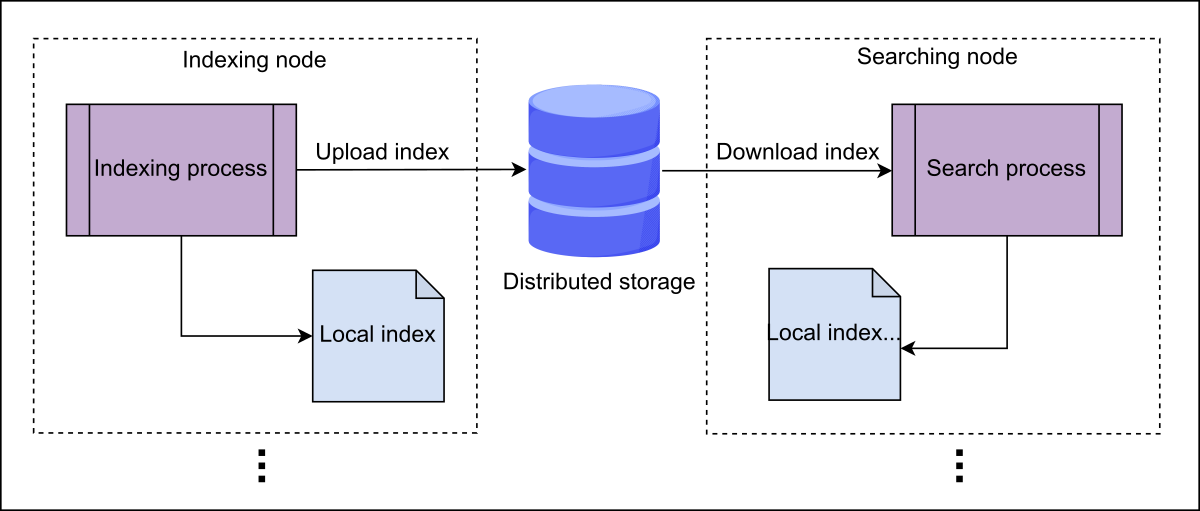
\includegraphics[width=0.5\textwidth]{Images/chapter_21/section_5899429382455296/5731941385371648.png}
 \caption{The indices produced by the indexing nodes are stored on the distributed storage, and the nodes involved in the search reads indices from the distributed storage to produce a result for the user's query}
\end{figure}

In the above illustration, a single node is shown for each indexing and searching operation. But , in reality, there would be an \protect\phantomsection\label{katex_inline_RWdPdCxcRNyLHMeN2p-kF}{{{\(N\)}}} number of nodes in the indexing phase, one node per partition (set of documents), that produces inverted indices. The inverted index is stored in the form of binary files on the nodes' local storage. Caching these blob files will result in performance improvement. These binary files are also pushed to a distributed storage. In the case of a hardware failure, a new searcher or indexer machine is added, and a copy of the data is retrieved from the distributed storage.
\\
When the upload is complete, the searcher nodes download the index files. Depending upon user search patterns, the searching nodes will maintain a cache of frequently asked queries and serve data from RAM. A user search query will be extended to all searcher nodes, which will generate responses according to their respective indices. A merger node in the front-end servers will combine all search results and present them to the user.
\\
The indexing process indexes the new documents as soon as they are available. At the same time, the searcher nodes fetch the updated indices to provide improved search results.

\subsection{Indexing explained}\label{ZfLDHAA69-1PvqoOzMmX7}
\\
Until now, we have explained the development of a highly scalable and performant design using low-cost nodes. However, we are unaware of the internals of the indexing nodes. In this section, we'll learn how indexing is performed with a MapReduce distributed model and parallel processing framework.
\\
The \textbf{MapReduce framework} is implemented with the help of a cluster manager and a set of worker nodes categorized as Mappers and Reducers. As indicated by its name, MapReduce is composed of two phases:

\begin{enumerate}
\item
\protect\phantomsection\label{9vxzd187y1CDxImIJfzj3}
The Map phase
\item
\protect\phantomsection\label{hGAR6MUtYcZKmRdNYepdy}
The Reduction phase
\end{enumerate}
\\
Furthermore, the input to MapReduce is a number of partitions, or set of documents, whereas its output is an aggregated inverted index.
\\
Let's understand the purpose of the above components:

\begin{itemize}
\item
\protect\phantomsection\label{mYnzrDTJnRPGHbmMu0fWz}
\textbf{Cluster manager}: The manager initiates the process by assigning a set of partitions to Mappers. Once the Mappers are done, the cluster manager assigns the output of Mappers to Reducers.
\item
\protect\phantomsection\label{ky0UKDP-cNB-LWDaiuDm2}
\textbf{Mappers}: This component extracts and filters terms from the partitions assigned to it by the cluster manager. These machines output inverted indexes in parallel, which serve as input to the Reducers.
\item
\protect\phantomsection\label{uSu3bdR64UfCoYj7m-W8O}
\textbf{Reducers}: The reducer combines mappings for various terms to generate a summarized index.
\end{itemize}
\\
The cluster manager ensures that all worker nodes are efficiently utilized in the cluster. The MapReduce is built to work under partial failures. If one node fails, it reschedules the work on another node.
\\
Note that the Reducers cannot start as long as the Mappers are working. This means that the cluster manager can use the same node as a Mapper as well as a Reducer.
\\
The slides below depict a simplified setup of how MapReduce can be used to generate an inverted index:

\begin{figure}[htbp]
 \centering
 \begin{subfigure}[b]{0.48\textwidth}
 \centering
 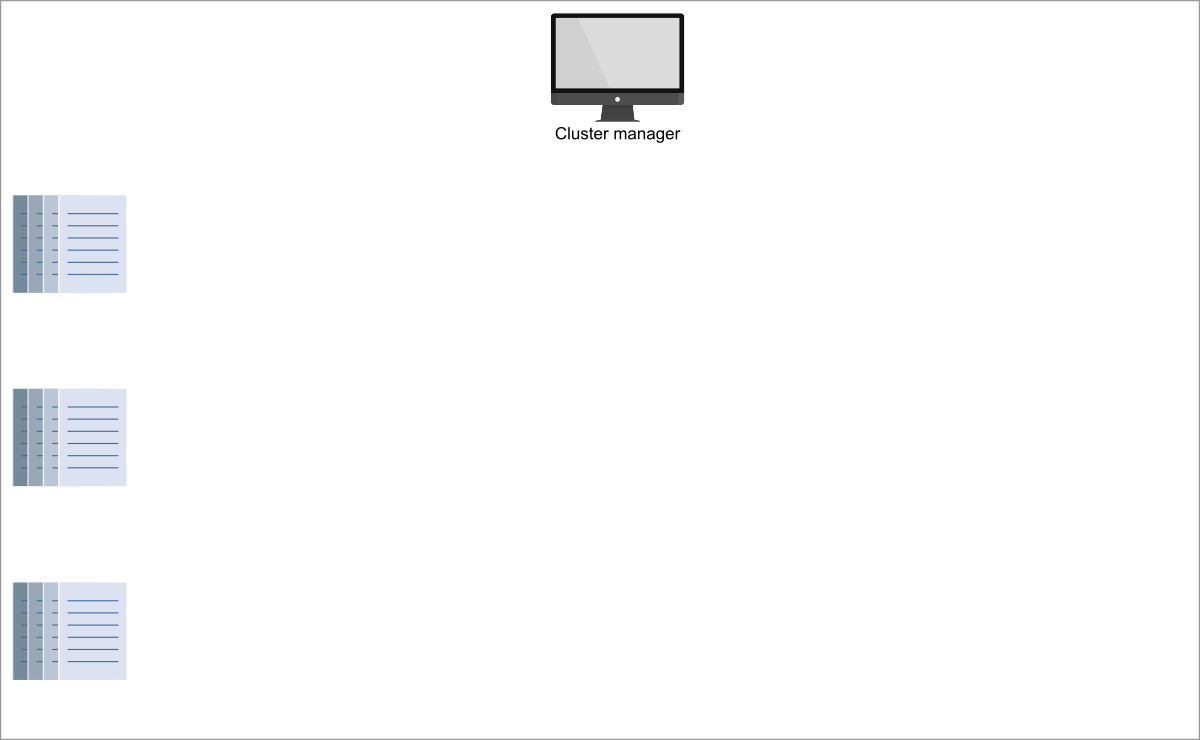
\includegraphics[width=\textwidth]{Images/chapter_21/section_5899429382455296/5086485997158400.png}
 \caption{ A cluster manager and document partitions}
 \end{subfigure}
 \hfill
 \begin{subfigure}[b]{0.48\textwidth}
 \centering
 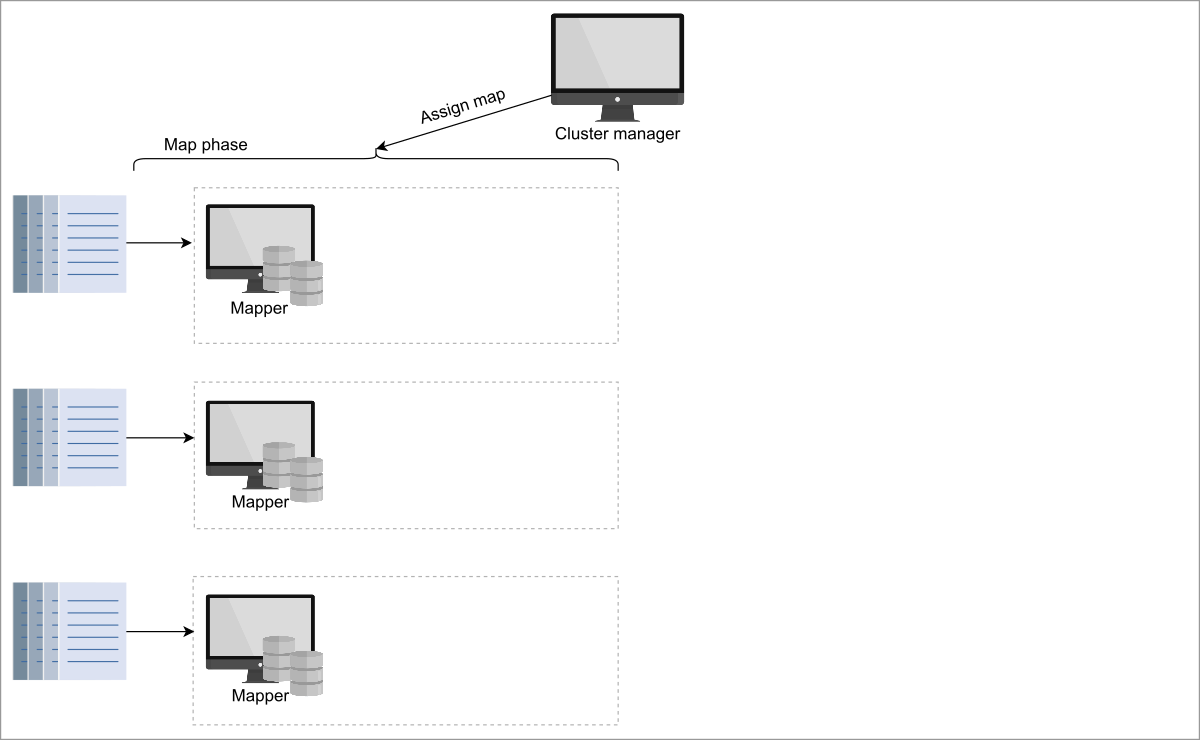
\includegraphics[width=\textwidth]{Images/chapter_21/section_5899429382455296/4522229861974016.png}
 \caption{The Map phase starts and the cluster manager assigns documents partitions to the idle nodes in the cluster. We call these nodes Mappers}
 \end{subfigure}
\end{figure}

\begin{figure}[htbp]
 \centering
 \begin{subfigure}[b]{0.48\textwidth}
 \centering
 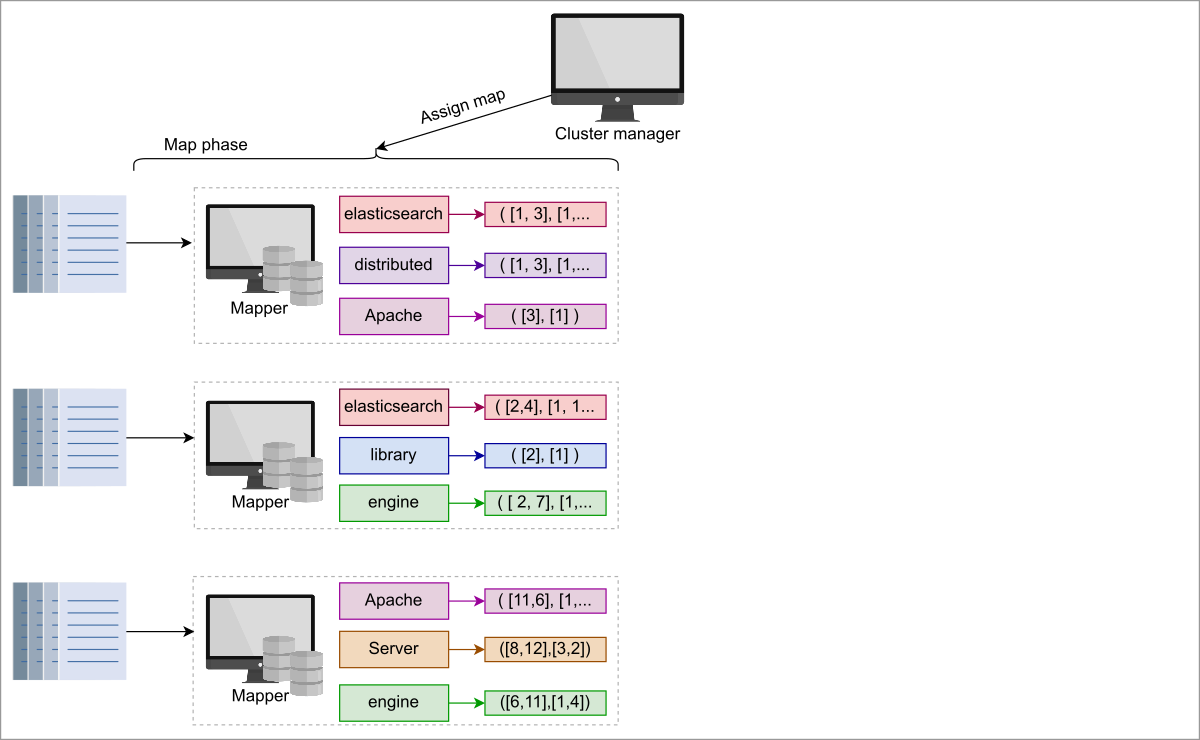
\includegraphics[width=\textwidth]{Images/chapter_21/section_5899429382455296/4577286275989504.png}
 \caption{Mappers extract terms from the assigned documents and produce N smaller inverted indices}
 \end{subfigure}
 \hfill
 \begin{subfigure}[b]{0.48\textwidth}
 \centering
 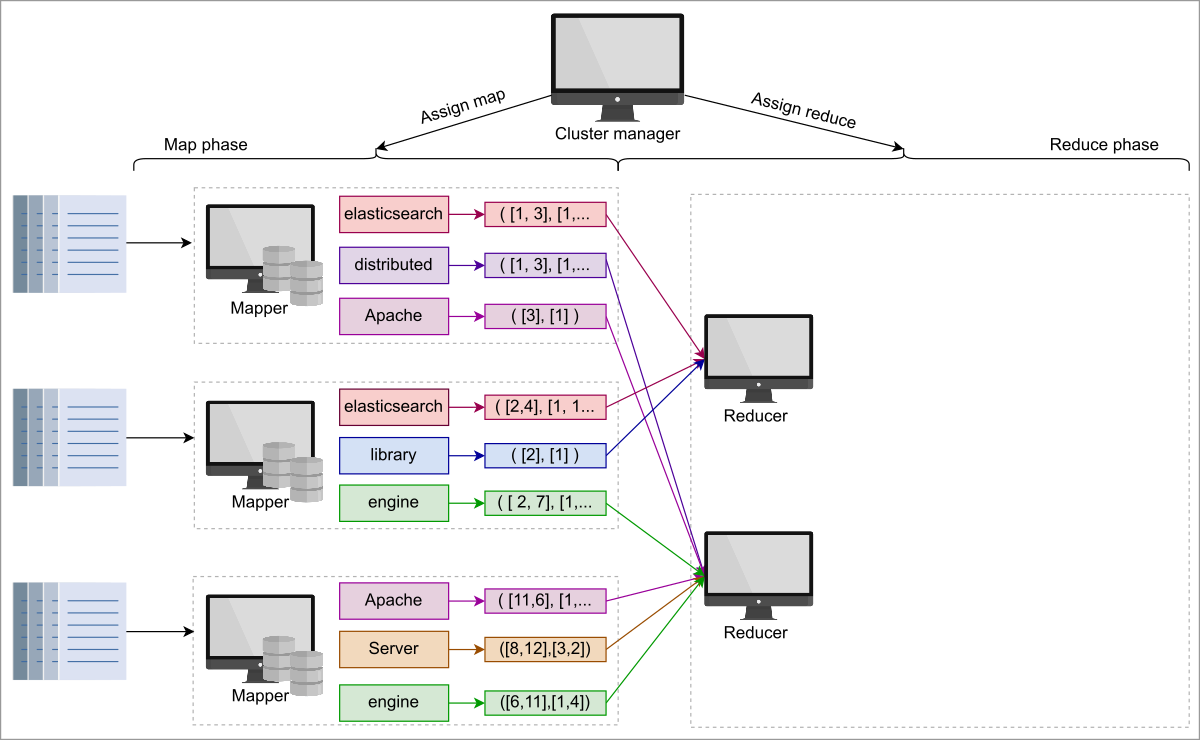
\includegraphics[width=\textwidth]{Images/chapter_21/section_5899429382455296/6671340799262720.png}
 \caption{The Reduce phase starts, the cluster manager identifies the idle nodes for running the Reduce function, and assigns work to the Reducers}
 \end{subfigure}
\end{figure}

\begin{figure}[htbp]
 \centering
 \begin{subfigure}[b]{0.48\textwidth}
 \centering
 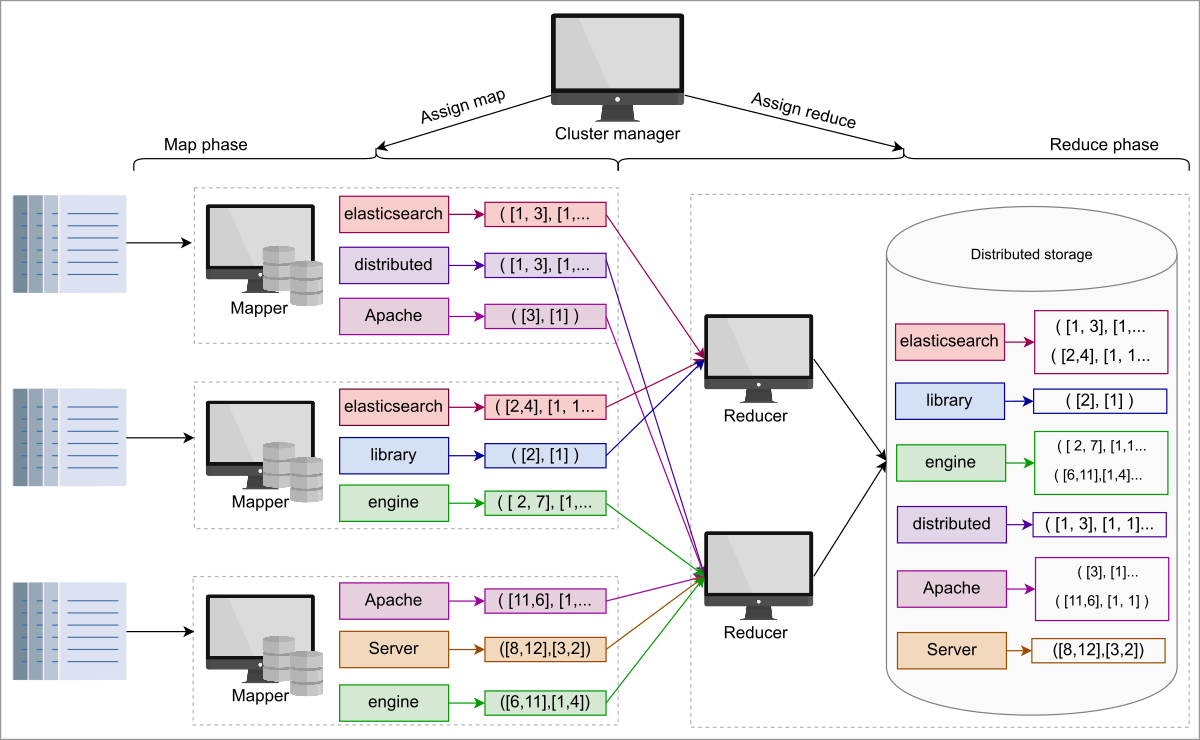
\includegraphics[width=\textwidth]{Images/chapter_21/section_5899429382455296/5417423964733440.png}
 \caption{The reducers combine similar terms from the assigned terms from all the mappers and put all the entries for a term together on the distributed storage}
 \end{subfigure}
\end{figure}

To keep it simple, we have just shown two indicators for each term in the above illustration: the list of documents in which the term appears and the list of the frequency of the term in each document (refer to \href{https://www.educative.io/courses/grokking-the-system-design-interview/indexing-in-a-distributed-search}{Indexing} for details).
\begin{quote}
\textbf{Note:} The above MapReduce setup is a simplified version of what happens in practice. A complex pipeline of the MapReduce framework is required to manage the complexities of a real-world search engine. However, the fundamental principles are the same as we presented here.
\end{quote}
\subsection{Summary}\label{xmoSSnyxDo_nHMr4GcF6f}
\\
In this lesson, we have resolved two key problems of scalability (due to colocated indexing and searching) and resource wastage (due to index recomputation) by using dedicated nodes for indexing and searching. Both operations rely on distributed storage. Furthermore , we presented a simplified description of the MapReduce framework to parallelize the indexing process.

% End of section content